\chapter{Introduction}\label{chapter:introduction}

New networking and cryptographic protocols can substantially improve
electronic online payment systems.  This book is about the design,
implementation and security analysis of GNU
Taler\footnote{\url{https://taler.net/}}, a privacy-friendly payment
system that is designed to be practical for usage as an online
(micro-)payment method, and at the same time socially and ethically
responsible.

Payment systems can generally be divided into two types: Register-based
and value-based~\cite{riksbank2017riksbank}.  A register-based system
associates value with identities (e.g., bank account balances with
customers), while a value-based system associates value with typically
anonymous, digital or physical tokens (such as cash or prepaid credit
cards).  In practice, these two types of systems are combined, as
different layers have different (and often conflicting) requirements:
the payment system used to pay for a cappuccino in a coffee shop is
most likely not suitable to buy real estate.  Value-based payment
systems typically provide more anonymity and convenience but also more
risk to consumers (as they are responsible to secure the values they
hold), while register-based systems shift risks to the payment service
provider who has to authenticate consumers and ensure the integrity of
the register.

This book explains GNU Taler, a design and implementation of a value-based
payment system, discussing in-depth how to create a practical,
privacy-preserving and secure (micro-)payment protocol that integrates nicely
with the modern web.  Our value-based payment protocol can in principle
operate on top of any existing register-based system.

GNU Taler is an official package of the GNU
project\footnote{\url{https://gnu.org/}}.  Our free software implementation is
freely available from the GNU mirrors.


\section{Design Goals for GNU Taler}

The design of payment systems shapes economies and societies
\cite{zandi2013impact,dalebrant2016monetary}.  Payment systems with high
transaction costs create an economic burden.  Predominantly cash-based
societies provide some degree of anonymity for their citizens, but can fail to
provide a sound foundation for taxation, facilitate corruption
\cite{singh2017does} and thus risk creating weak governments. On the other
hand, systems with too much surveillance eliminate personal freedom.

As the Internet has no standardized payment system, especially not one
that is capable of quickly, efficiently and securely settling small
transactions (so-called micropayments), the majority of content on the web is
financed by advertisements.  As a result, advertising (and by
implication, collecting data on users) has been a dominant business
model on the Internet.  This has not only resulted in a loss of
independence of publishers---who need to cater to the needs
of advertisers---but also in a situation where micro-targeted ads
are so wide-spread, that they have been suspected to have influenced
multiple major elections~\cite{persily2017election}.  Ads are also a
vector for malware \cite{provos2007ghost}.  Due to the prevalence of
ad blockers, ads are also not guaranteed to be a sustainable business
model.

In the world of online payments, credit cards and a sprawling number
of smaller, proprietary payment processors are currently dominant, and
market shares vary widely between different
countries~\cite{adyen2016global,paypers2016ecommerce}.  The resulting
fragmentation again increases social costs: online shops can either
choose to invest in implementing many proprietary protocols, or only
implement the most popular ones, thereby reinforcing the dominance of
a handful of proprietary payment systems.

Considering these and other social implications of payment systems, we
started the development of GNU Taler with a set of high-level design
goals that fit our social agenda.  They are ranked by the importance
we give to them, and when a trade-off must be made, the one that
supports the more highly ranked goal is preferred:

% what about micropayments -> part of 'efficient'
\begin{enumerate}
  \item \textbf{GNU Taler must be implemented as free software.}

    Free refers to ``free as in free speech'', as opposed to ``free as in free beer''.
    More specifically, the four essential freedoms of free software
    \cite{stallman2002essays} must be respected, namely users must have the
    freedom to (1) run the software, (2) study and modify it, (3) redistribute
    copies, and (4) distribute copies of the modified version.

    For merchants this prevents vendor lock-in, as another payment provider can
    take over, should the current one provide inadequate quality of service.
    As the software of
    the payment provider itself is free, smaller or disadvantaged countries or
    organizations can run the payment system without being controlled by a
    foreign company.  Customers benefit from this freedom, as the wallet
    software can be made to run on a variety of platforms, and user-hostile
    features such as tracking or telemetry could easily be removed from
    wallet software.

    This rules out the mandatory usage of specialized
    hardware such as smart cards or other hardware security modules, as the
    software they run cannot be modified by the user.  These components can,
    however, be voluntarily used by merchants, customers or payment processors
    to increase their operational security.

  \item \textbf{GNU Taler must protect the privacy of buyers.}\label{item:privacy}

    Privacy should be guaranteed via technical measures, as opposed to mere
    policies.  Especially with micropayments for online content, a
    disproportionate amount of rather private data about buyers would be revealed, if
    the payment system does not have privacy protections.

%Especially if a payment system is to be used for microtransactions for online
%content, the privacy of buyers becomes important: if micropayments were more
%commonplace, the transaction data could be used to collect extremely detailled
%profiles of users.  Unfortunately practically no commercially used payment
%system has strong anonymity guarantees.
    
    In legislations with data protection regulations (such as the recently introduced GDPR in Europe \cite{voigt2017eu}),
    merchants benefit from this as well, as no data breach of customers can happen if this information
    is, by design, not collected in the first place.  Obviously some private data, such as the shipping
    address for a physical delivery, must still be collected according to business needs.

    The security of the payment systems also benefits from this, as the model
    shifts from authentication of customers to mere authorization of payments.
    This approach rules out whole classes of attacks such as phishing \cite{garera2007framework} or credit
    card fraud \cite{sahin2010overview}.

  \item \textbf{GNU Taler must enable the state to tax income and crack down on
    illegal business activities.}

    % FIXME: provide broader ethical justification!
    As a payment system must still be legal to operate and use, it must comply
    with these requirements.  Furthermore, we consider levying of taxes as
    beneficial to society.

  \item \textbf{GNU Taler must prevent payment fraud.}

    This imposes requirements on the security of the system, as well as on the
    general design, as payment fraud can also happen through misleading user
    interface design or the lack of cryptographic evidence for certain
    processes.

  \item \textbf{GNU Taler must only disclose the minimal amount of information
    necessary.}

    The reason behind this goal is similar to (\ref{item:privacy}).  The
    privacy of buyers is given priority, but other parties such as merchants
    still benefit from it, for example, by keeping details about the merchant's financials
    hidden from competitors.


  \item \textbf{GNU Taler must be usable.}

    Specifically it must be usable for non-expert customers.  Usability also
    applies to the integration with merchants, and informs choices about the
    architecture, such as encapsulating procedures that require cryptographic
    operations into an isolated component with a simple API.

  \item \textbf{GNU Taler must be efficient.}

    % FIXME: provide broader ethical justification (environmental impact,
    % social cost, opportunity cost of lack of micropayments)
    Approaches such as proof-of-work are ruled out by this requirement.  Efficiency is
    necessary for GNU Taler to be used for micropayments.

  \item \textbf{GNU Taler must avoid single points of failure.}

    While the design we present later is rather centralized, avoiding single
    points of failure is still a goal.  This manifests in architectural choices such as
    the isolation of certain components, and auditing procedures.

  \item \textbf{GNU Taler must foster competition.}

    It must be relatively easy for competitors to join the systems.  While the
    barriers for this in traditional financial systems are rather high, the
    technical burden for new competitors to join must be minimized. Another
    design choice that supports this is to split the whole system into smaller
    components that can be operated, developed and improved upon independently,
    instead of having one completely monolithic system.

\end{enumerate}



\section{Features of Value-based Payment Systems}\label{sec:intro:features}

There are many different possible features that have been proposed for
value-based (sometimes called token-based) payment systems in the past.  While we
will discuss existing work on e-cash in more detail in
Section~\ref{sec:related-work:e-cash}, we will begin by a brief
summary of the possible features that value-based payment systems
could provide, and clarify which high-level features we chose to adopt
for GNU Taler.

% EXPLAIN:  in traditional (online) e-cash, spending is never
% bound to a contract identifier

%\subsubsection*{Different signature schemes and zero-knowledge proofs}
%Since Chaum's original blind signature scheme based on RSA, many variations
%using other cryptographic primitives have been developed.  Some newer e-cash
%schemes do not use blind signatures, but rely on zero-knowledge proofs instead.
%
%In GNU Taler, we opt for an RSA-based blind signature scheme, due to the low
%complexity, relatively clear security assumptions and small number of
%communication rounds compared to other protocols.

\subsection{Offline vs Online Payments}

Anonymous digital cash schemes since Chaum~\cite{chaum1983blind} were frequently designed to allow
the merchant to be offline during the transaction, by providing a means to
deanonymize customers involved in double-spending, typically by encoding the
customer's identity into their coins in a way that makes it only possible to
decode the identity with two spending transcripts.

This approach is problematic in practice, as customers that restore a wallet
from backup might accidentally double-spend and would then face punishment for
it.  Enforcing punishment for double-spenders can be rather difficult as well,
since the double-spender might have signed up with a false identity or might
already have fled to another country, and a large number of merchants might already
have been defrauded with the same coins.

Should the issuer of e-cash be compromised, an attacker could issue coins that
fail to identify a culprit or even blame somebody else when they are
double-spent.  In an offline e-cash system, the detection of such an event is
greatly delayed compared to systems with online spending, which can immediately
detect when more coins are spent than were issued.

Thus, in GNU Taler, we decided that all coins must be immediately
deposited online during a purchase.  Only either a merchant or a customer
needs to be online, since one of the two can forward messages to the
payment service provider for the other.

\subsection{Change and Divisibility}

Customers  do not always have the right set of coins available to exactly cover
the amount to be paid to a merchant.  With physical cash, the store would
give the customer change.  For e-cash, the situation is more complex, as
the customer would have to make sure that the change has not already been
spent, does not violate their anonymity and the merchant does not have a
digital ``copy'' of the change tokens that the merchant can spend before the customer.  Note
that it would be unwise to always withdraw the correct amount of e-cash
directly before a purchase, as it creates a temporal correlation between the
non-anonymous withdrawal event and the spending event.

Most modern e-cash schemes instead deal with exact spending  by providing
\emph{divisibility} of coins, where the customer can decide to only spend part
of a coin.  A significant chunk of the e-cash literature has been concerned
with developing schemes that allow the individual, divided parts of a coin to
be unlinkable (thus preserving anonymity) and to optimize the storage costs for
wallets and the communication cost of withdrawals.

The current state of the art for divisible e-cash~\cite{pointcheval2017cut}
achieves constant-time withdrawal and wallet storage cost for coins that can be
split into an arbitrary but fixed (as a system parameter) number of pieces.  A
continuous ``chunk'' of the smallest pieces of a coin can be spent with
constant-time communication complexity.

While this sounds attractive in theory, these results are mostly of academic
interest, as the storage and/or computational complexity for the party that is
checking for double spending of coins remains enormous:  each smallest piece of
every coin needs to be recorded and checked individually.  When paying
$\$10.00$ with a coin that supports division into cent pieces, $1000$
individual coin pieces must be checked for double spending and recorded,
possibliy in compressed form to trade storage costs for more computation.

For GNU Taler, we use a rather simple and practical approach, made possible by
requiring participants to be online during spending:  coins can be fractionally
spent without having divisible, unlinkable parts. The remaining value on a coin
that was spend (and thus revealed) can be used to withdraw fresh, unlinkable
coins.  The protocol to obtain change takes additional measures to ensure that
it cannot be misused to facilitate untaxed transactions.  Giving change for
e-cash has been proposed before \cite{brickell1995trustee,tracz2001fair}, but
to the best of our knowledge, the idea of income-transparent change is novel.

\subsection{Anonymity Control}

Some proposed e-cash protocols contain mechanisms to allow selective
deanonymization of transactions for scenarios involving crime
\cite{sander1999escrow}, specifically blackmailing and tax evasion.

Unfortunately this does not really work as a countermeasure against
blackmailing in practice.  As noted in the paper that initially described such
a mechanism for blind signatures \cite{stadler1995fair}, a blackmailer could
simply request to be paid directly with plain, blindly signed coins, and
thereby completely circumvent the threat of revocable anonymity.

GNU Taler provides \emph{income transparency} as a measure against tax evasion.
We furthermore describe a different approach in a blackmailing scenario in
Section~\ref{sec:design:blackmailing}, which we believe is more practical in
dissuading blackmailers in practice.

\subsection{User Suspension}

Anonymous user suspension \cite{au2011electronic} has been proposed as
another mechanism to punish users suspected in illicit activities by
preventing then from making further transactions until the suspension is
lifted.  Anonymous suspension is based on transactions; the user
involved in a particular transaction is suspended, but their identity is not
revealed.

While the approach is interesting, it is not practical, as it requires
a single permanent key pair to be associated with each user.  If a
user claims they lost their private key and requests a new key pair,
their suspension would be effectively lifted. Suspending users from a
dominant payment system is also socially problematic, as excluding
them from most commercial activities would likely be a
disproportionate and cruel punishment.

\subsection{Transferability}

Transferability is a feature of certain e-cash systems that allows
transfer of e-cash between two parties without breaking anonymity
properties \cite{fuchsbauer2009transferable}.  Contemporary systems
that offer this type of disintermediation attract criminal
activity~\cite{richet2016extortion}.

GNU Taler specifically provides roughly the \emph{opposite} of this property,
namely \emph{income transparency}, to guarantee that e-cash is not easily
abused for tax evasion.  Mutually trusting users, however, can share ownership
of a coin.

\subsection{Atomic Swaps}

Atomic swaps (often called ``fair exchange'' in the e-cash literature) are a
feature of some e-cash systems that allows e-cash
to be exchanged against some service or (digital) product, with a trusted third
party ensuring that the payee receives the payment if and only if they correctly
provided the merchandise.

GNU Taler supports Camenisch-style atomic swaps~\cite{camenisch2007endorsed},
as explained in Section~\ref{sec:security:atomic-swaps}.

\subsection{Refunds}

GNU Taler allows merchants to provide refunds to customers during a limited
time after the coins for the payment were deposited.  The merchant signs a
statement that effectively allows the customer to reclaim a previously spent
coin.  Customers can request anonymous change for the reclaimed amount.

While this is a rather simple extension, we are not aware of any other e-cash
system that supports refunds.


\section{User Experience and Performance} \label{sec:intro:ux}

For adoption of a payment system, the user experience is critical. Thus,
before diving into {\em how} GNU Taler is implemented, we begin by 
showing how GNU Taler {\em looks} from the perspective of an end user in the
context of web payments, in a desktop browser (Chromium).

To use GNU Taler, the user must first install a browser extension
(Figure~\ref{fig:ux:install-prompt}).  Once installed, the user can
open a pop-up window by clicking on the Taler logo, to see the
initially empty wallet balance (Figure~\ref{fig:ux:installed}).

The customer logs into their online bank---a simple demo bank in our case--to
withdraw digital cash from their bank account into their wallet (Figures~%
\ref{fig:ux:bank-login} and~\ref{fig:ux:bank-profile}).  Our demo uses
\textsc{Kudos} as an imaginary currency.  Before the user is asked to confirm,
they are given the option to view details about or change the default exchange
provider, the GNU Taler payment service provider (Figure~\ref{fig:ux:select-exchange}).

With a real bank, a second factor (such as a mobile TAN) would now be requested
from the user.  Our demo instead asks the user to solve a simple CAPTCHA
(Figure~\ref{fig:ux:pin-tan}).  The amount withdrawn---minus withdrawal
fees---is now available as e-cash in the wallet (Figure~%
\ref{fig:ux:withdraw-done}).

The customer can now go to an online shop to spend their digital cash.  We've
implemented a shop that sells single chapters from Richard Stallman's essay
collection ``Free Software, Free Society'' \cite{stallman2002essays} (Figure~%
\ref{fig:ux:essay-landing}).  The user selects an essay, and is then
immediately presented with a confirmation page rendered by the wallet (Figure~\ref{fig:ux:essay-pay}).
After paying, the user can immediately read the article (Figure~\ref{fig:ux:essay-done}).

Our benchmarks, discussed in Chapter \ref{chapter:implementation} show that a
single machine can support around 1000 payments per second, and our
implementation is easily amenable to further scaling.

The extra computation required in the customer's wallet is in the order of a
few hundred milliseconds even on typical mobile or tablet devices, and thus
barely noticeable.

\begin{figure}
\centering
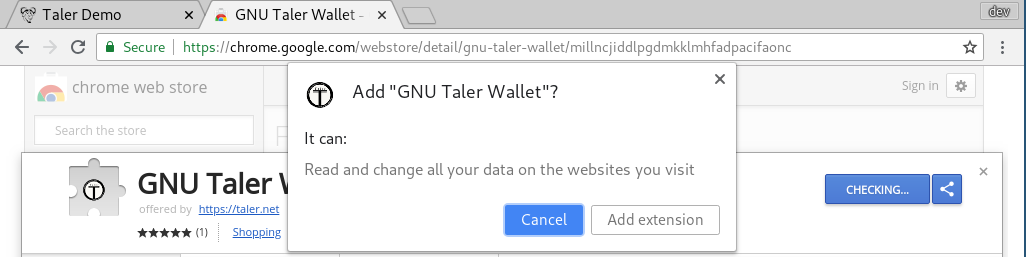
\includegraphics[width=\textwidth]{taler-screenshots/wallet-install-prompt.png}
\caption{The user is prompted to install the wallet.}
\label{fig:ux:install-prompt}
\end{figure}

\begin{figure}
\centering
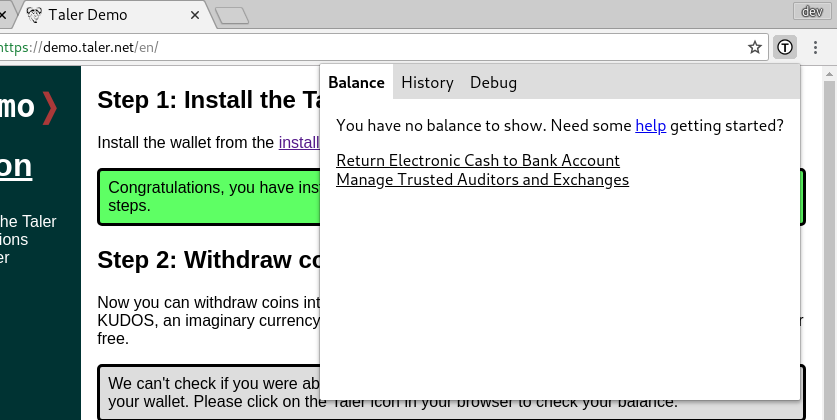
\includegraphics[width=\textwidth]{taler-screenshots/wallet-installed.png}
\caption{The wallet popup shows an empty balance.}
\label{fig:ux:installed}
\end{figure}

\begin{figure}
\centering
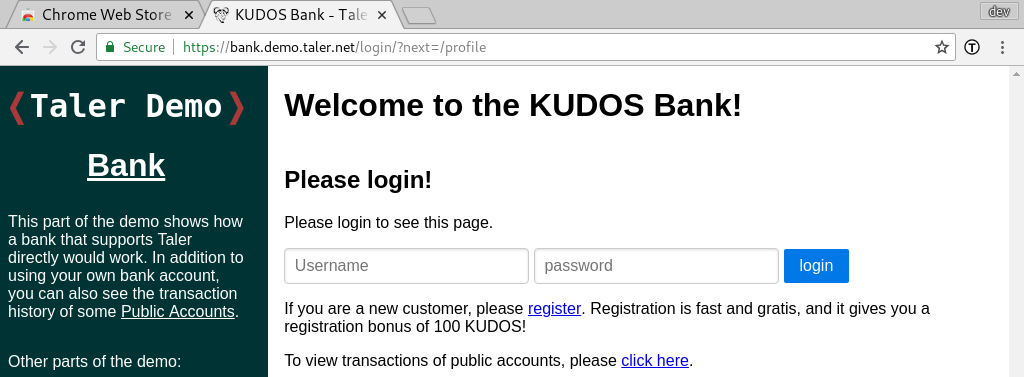
\includegraphics[width=\textwidth]{taler-screenshots/bank-login.png}
\caption{The bank asks for login details.}
\label{fig:ux:bank-login}
\end{figure}

\begin{figure}
\centering
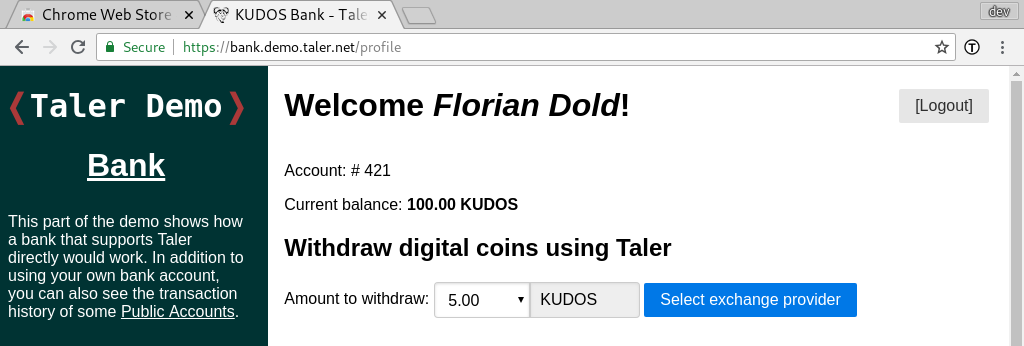
\includegraphics[width=\textwidth]{taler-screenshots/bank-profile.png}
\caption{Account page of the demo bank.}
\label{fig:ux:bank-profile}
\end{figure}

\begin{figure}
\centering
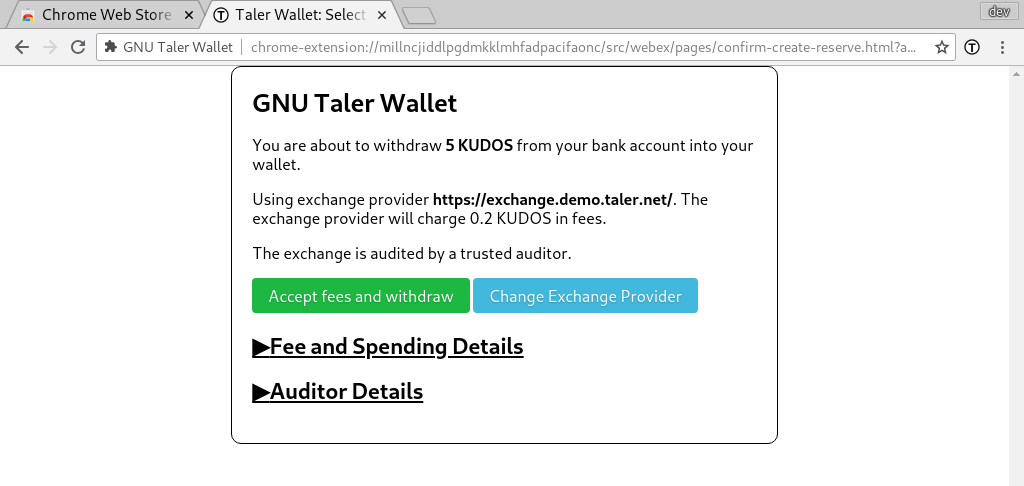
\includegraphics[width=\textwidth]{taler-screenshots/withdraw-confirm.png}
\caption{Exchange selection dialog in the wallet.}
\label{fig:ux:select-exchange}
\end{figure}

\begin{figure}
\centering
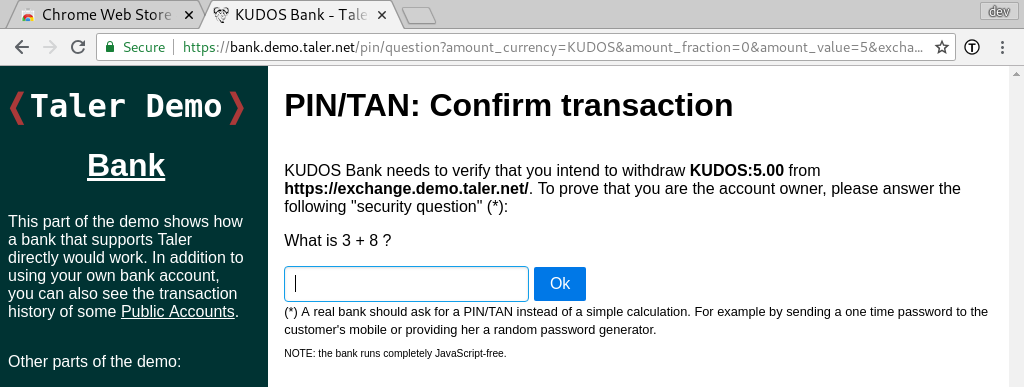
\includegraphics[width=\textwidth]{taler-screenshots/pin-tan.png}
\caption{PIN/TAN dialog of the demo bank.}
\label{fig:ux:pin-tan}
\end{figure}

\begin{figure}
\centering
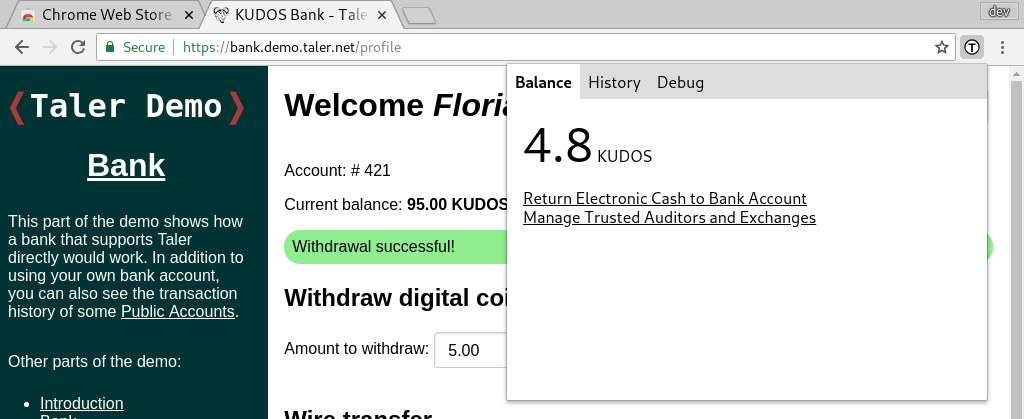
\includegraphics[width=\textwidth]{taler-screenshots/withdraw-done.png}
\caption{After a successful withdrawal, the balance is shown in the wallet.}
\label{fig:ux:withdraw-done}
\end{figure}

\begin{figure}
\centering
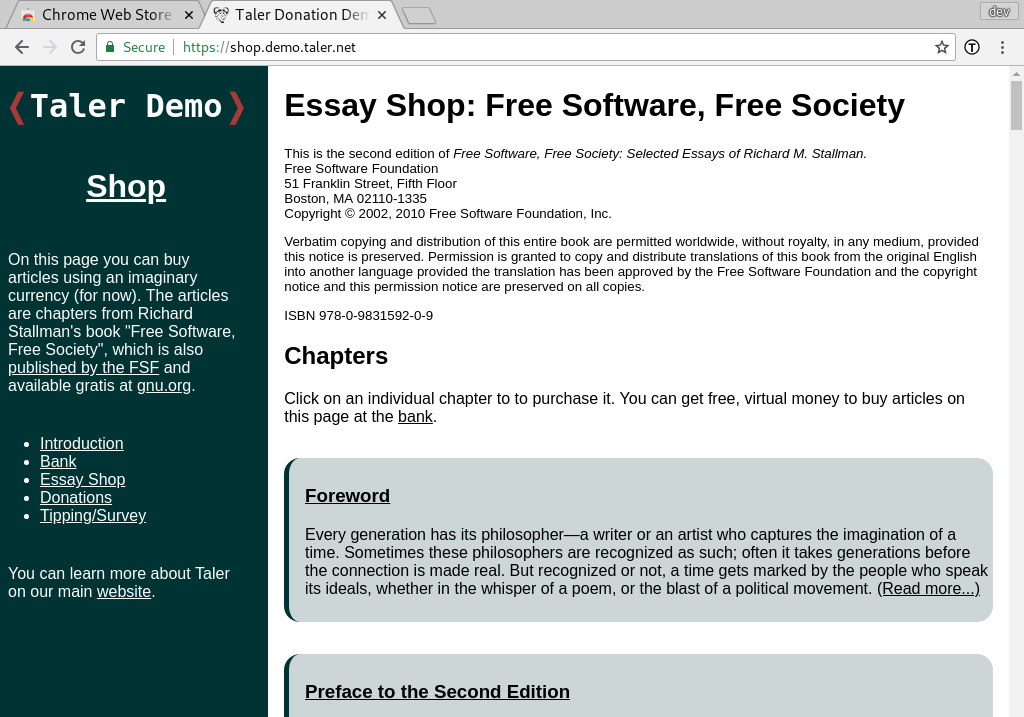
\includegraphics[width=\textwidth]{taler-screenshots/essay-landing.png}
\caption{Landing page of a store that sells essays.}
\label{fig:ux:essay-landing}
\end{figure}

\begin{figure}
\centering
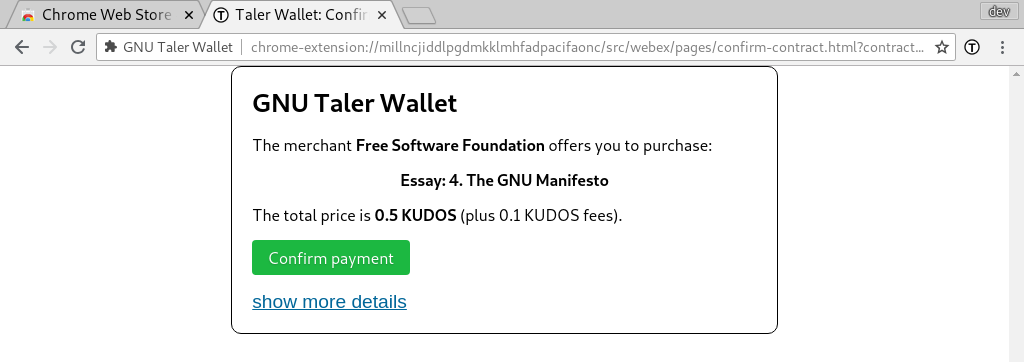
\includegraphics[width=\textwidth]{taler-screenshots/essay-pay.png}
\caption[Payment prompt for an essay.]{Payment prompt for an essay.  Rendered by the wallet.}
\label{fig:ux:essay-pay}
\end{figure}

\begin{figure}
\centering
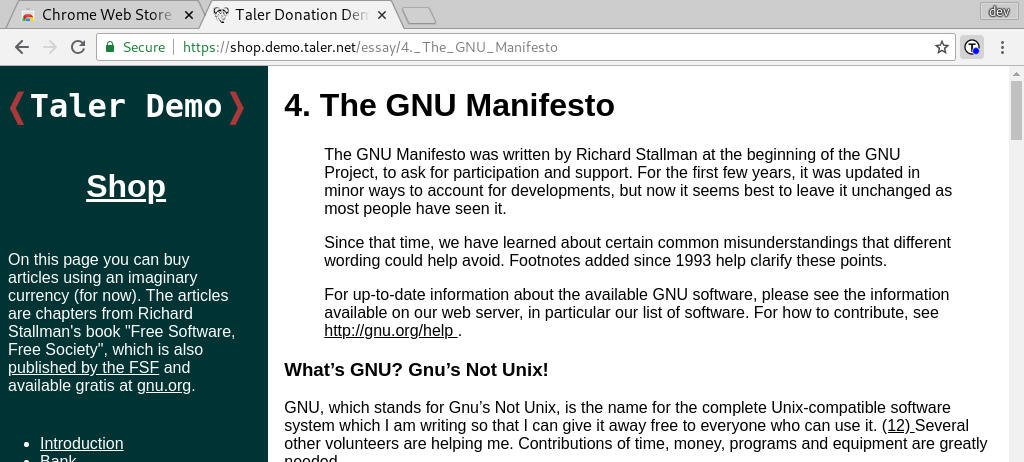
\includegraphics[width=\textwidth]{taler-screenshots/essay-done.png}
\caption{Essay successfully purchased by the user.}
\label{fig:ux:essay-done}
\end{figure}

%\begin{figure}
%\begin{subfigure}{.5\textwidth}
%  \centering
%  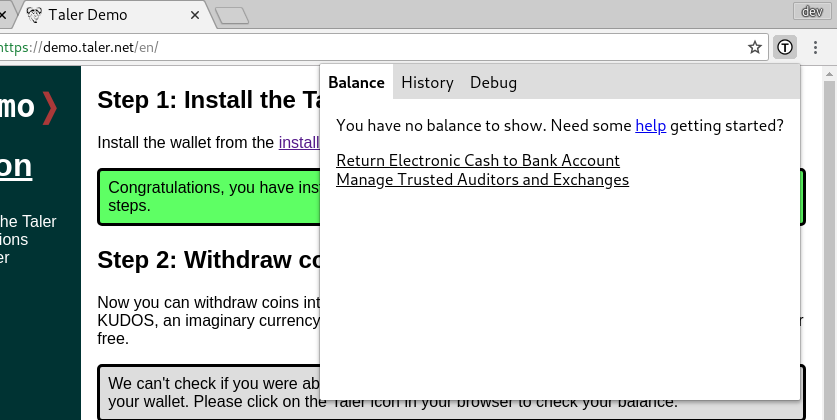
\includegraphics[width=.8\linewidth]{taler-screenshots/wallet-installed.png}
%  \caption{1a}
%  \label{fig:sfig1}
%\end{subfigure}%
%\begin{subfigure}{.5\textwidth}
%  \centering
%  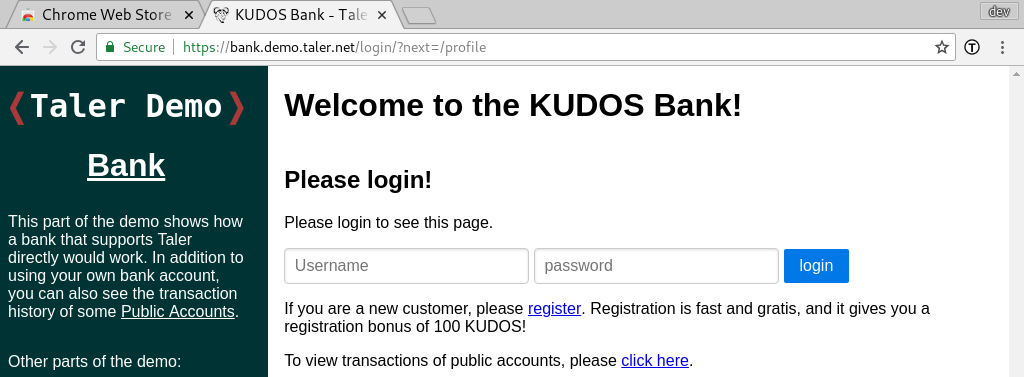
\includegraphics[width=.8\linewidth]{taler-screenshots/bank-login.png}
%  \caption{1b}
%  \label{fig:sfig2}
%\end{subfigure}
%\caption{plots of....}
%\label{fig:fig}
%\end{figure}

% FIXME: perf results

\section{The Technical Foundation: Anonymous E-Cash} \label{sec:intro:ecash}
GNU Taler is based on anonymous e-cash.  Anonymous e-cash was invented by David
Chaum in the 1980s \cite{chaum1983blind}.  The idea behind Chaumian e-cash is
both simple and ingenious, and can be best illustrated
with the carbon paper\footnote{%
  Carbon paper is a paper coated with pigment (originally carbon) on one side.
  When put face-down between two sheets of normal paper, the pressure from
  writing with a pen or typewriter on the first layer causes pigment to be
  deposited on the paper beneath, allowing a copy to be made.
} analogy:  A long, random serial number is generated, for example, by throwing
a die a few dozen times, and written on a piece of paper.  A carbon paper is
placed on top, with the pigmented side facing down, and both pieces of paper
are put into an opaque envelope.  The envelope is now sealed and brought to a
bank.  The bank draws a signature on the outside of the envelope, which presses
through to the piece of paper with the serial number.  In exchange for the
signed envelope, the bank deducts a fixed amount (say five dollars) from the
customer's bank account.  Under the (admittedly rather strong) assumption that
the bank's signature cannot be forged, the signed piece of paper with the serial
number is now an untraceable bank note worth five dollars, as the bank signed
it without seeing the serial number inside the envelope!  Since the signed
paper can be easily copied, merchants that accept it as payment must check the
bank's signature, call the bank and transmit the serial number.  The bank keeps
a register of all serial numbers that have been used as payment before.  If the
serial number is already in the bank's register, the bank informs the merchant
about the attempted double spending, and the merchant then rejects the payment.

The digital analogue of this process is called a \emph{blind signature}, where
the signer knows that it gave a digital signature, but does not know the
contents of the message that it signed.

In this document, we use \emph{coin} to refer to a token of value in an e-cash
system.  Note that the analogy of a coin does not always hold up, as certain
types of operations possible in some e-cash schemes, such as partial spending,
divisibility, etc., do not transfer to physical coins.


%\subsection{Security Properties}\label{sec:intro:security}

We have the following security and correctness properties for GNU Taler
(formally defined in Chapter~\ref{chapter:security}):
\begin{itemize}
  \item \emph{Anonymity} guarantees that transactions cannot be correlated with withdrawals or
    other transactions made by the same customer.
  \item \emph{Unforgeability} guarantees that users cannot spend more e-cash than they withdrew.
  \item \emph{Conservation} guarantees that customers do not lose money due to
    interrupted protocols or malicious merchants; they can always obtain
    anonymous change or a proof of successful spending.
  \item \emph{Income transparency} guarantees that mutually distrusting parties
    are unable to reliably transfer e-cash between them without the income of
    participants being visible to tax auditors.
\end{itemize}

While anonymity and unforgeability are common properties of e-cash, we are not
aware of any other treatments of income transparency and conservation.


\section{Roadmap}

Chapter \ref{chapter:design} describes the high-level design of GNU Taler, and
compares it to payment systems found in the academic literature and real-world
usage.  Chapter \ref{chapter:security} first gives a gentle introduction to
provable security (which can be skipped by readers with a background in
cryptography), and then defines security properties for income-transparent,
anonymous e-cash.  The cryptographic protocols for GNU Taler are defined in
detail, and proofs are given that our protocols satisfy the security
properties defined earlier.  In Chapter \ref{chapter:implementation}, the
implementation of GNU Taler is described, and the performance and scalability
is evaluated.  Chapter \ref{chapter:future-work} discusses future work and
missing pieces to deploy GNU Taler in production.  Chapter
\ref{chapter:conclusion} concludes with an outlook on the potential impact and
practical relevance of this work.

